\documentclass[10pt,a4paper,oneside]{book}

\begin{document}

\chapter{Laboratory Instructions}

\section{Materials}

\begin{itemize}
    \item{Sample to image (cells, DNA origami, etc.)}
    \item{Imaging buffer (Abbelight Smart Kit for STORM)}
    \item{Cavity well microscope slide}
    \item{Sealant}
    \item{Immersion oil}
    \item{Lens cleaning solution (ethanol, etc.)}
\end{itemize}

\section{Description of the Microscope}

The microscope is an Abbelight SAFe 180. It consists of an Olympus IX83 microscope, an Abbelight scanning illumination system, an Oxxius laser engine, a Hamamatsu ORCA-Fusion digital CMOS camera, and other components. Some of these components are labeled in \autoref{fig:microscope} and \autoref{fig:electronics}.

\begin{figure}[ht]
    \centering
    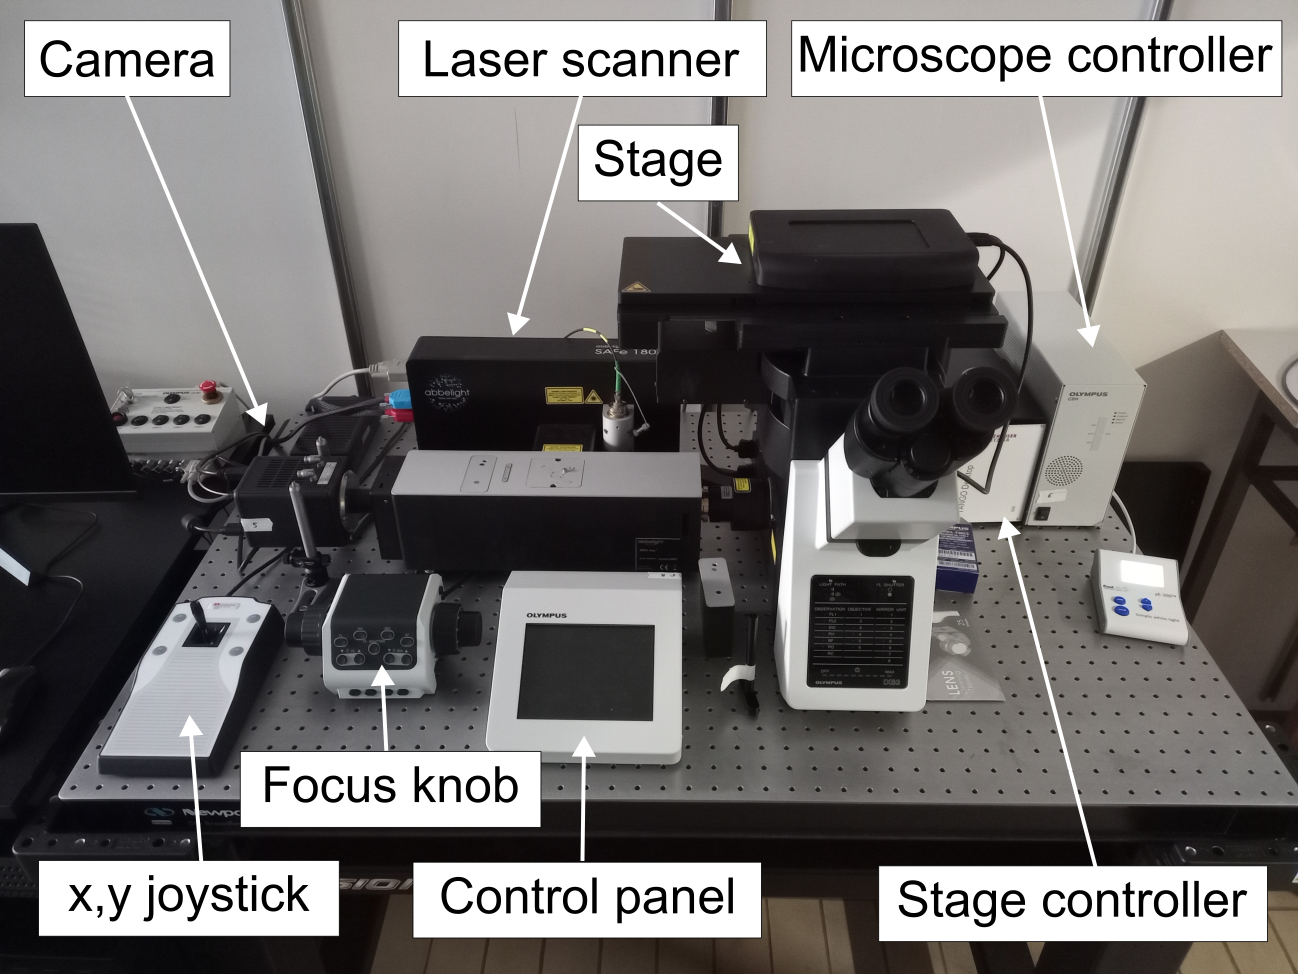
\includegraphics[width=0.75\textwidth]{microscope.png}
    \caption{The primary components of the microscope used in this course.}
    \label{fig:microscope}
\end{figure}

\begin{figure}[ht]
    \centering
    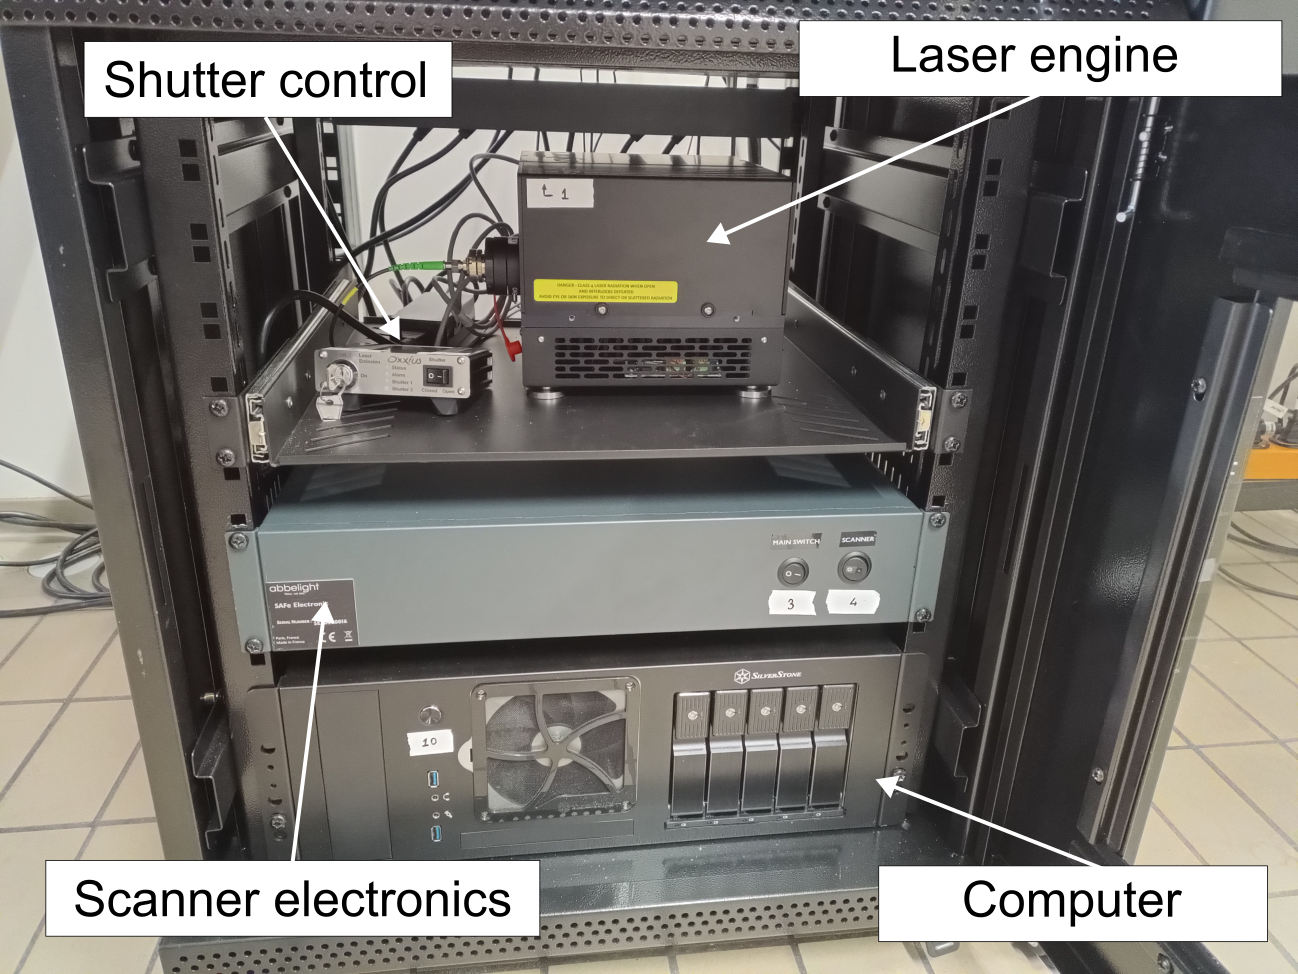
\includegraphics[width=0.75\textwidth]{electronics.png}
    \caption{Electronics and laser source for the microscope.}
    \label{fig:electronics}
\end{figure}

\section{Tasks}

\subsection{Turn on the Microscope}\label{sec:startup}

To turn on the microscope, switch on the following components in this order. There should be pieces of tape with numbers on them and attached to the actual devices to aid you.

\begin{enumerate}
    \item Laser engine
    \item Laser safety key on the shutter controller
    \item Scanner electronics: main switch
    \item Scanner electronics: scanner
    \item Camera \newline Wait for the status light to turn green before proceeding.
    \item Olympus CBH microscope controller
    \item Maerhaeuser Tango Desktop stage controller
    \item Olympus control panel \newline Wait for the "Start Operation" button to appear, then press it to continue. This can take about one minute.
    \item Laser shutter
    \item The computer
\end{enumerate}

\subsection{Prepare the Buffer}

\fbox{
    \parbox{\textwidth}{\textbf{WARNING} The buffers used in SMLM contain highly toxic chemicals. Always follow proper laboratory safety procedures. Please alert a teaching assistant immediately if any of the buffer touches you.}
}\newline

For STORM imaging, the sample must be immersed in a buffer that facilitates photoswitching. Follow the instructions in the Abbelight Smart Kit to prepare the buffer.

\subsection{Prepare the Sample}

Once the buffer is prepared, remove the sample that you will image from the fridge. If it is a cell sample, then it will be mounted on a glass coverslip that must in turn be mounted onto a microscope slide with a well to hold the buffer. Carefully add the buffer to the well and \textbf{place the coverslip with the sample slide facing the buffer} over the well.

\subsection{Mount the Sample onto the Microscope}

\subsection{Find a Region to Image}

After mounting the sample, you should start the imaging software which is called \textbf{NEO Live Imaging}. You will see a screen like the one in \autoref{fig:liveimaging-startup}.

\begin{figure}[ht]
    \centering
    
\includegraphics[width=1.0\textwidth]{liveimaging-startup.png}
    \caption{The NEO Live Imaging screen immediately after startup.}
    \label{fig:liveimaging-startup}
\end{figure}

\subsection{Shutdown the Microscope}

Turn off the components in the opposite order as in \autoref{sec:startup}.

\subsection{Clean Remove Oil From the Objective}

The oil must be removed from the objective after imaging, and sometimes during imaging if there is dust in the oil. To do this, use lens cleaning solution and lens tissue to clean the objective. The lens tissue should be folded into a small square and wetted with the cleaning solution. Avoid touching the area of the tissue that you will use to clean the objective. Then, gently wipe the objective with the wetted lens tissue, slowly dragging the tissue across the objective in one direction.

A video demonstration on cleaning objectives may be found at \url{https://www.youtube.com/watch?v=Tz4Dy5D6kdw}.

\end{document}
